\section{The warp rule on a fixed camera is the range rule}
\label{app:parity}

With the identity warp, no per-patch refinement and a canvas written only at whole pixel positions, every read in \eqref{eq:W} lands on a canvas pixel with weight one, and every canvas pixel holds the value of the frame that last kept it, unresampled. Then $W = R$, the last copy sent, on every patch, $\iota \equiv 0$, and the warp rule's statistic is the range rule's. The repository checks this bit for bit: on a synthetic fixed-camera sequence with noise and a planted change, the keep masks of the two implementations are identical, their scores agree to floating-point precision, and the maximum of $\iota$ is exactly zero (test \texttt{test\_fixed\_camera\_is\_the\_range\_rule\_bit\_for\_bit} in \texttt{tests/test\_paper.py}).

\section{What each reducer re-implementation keeps}
\label{app:reducers}

Each rule maps frames and a threshold to a keep mask over patches and frames, with frame~0 kept, so that one calibration routine can set every rule to the same budget. None of them is the published system: the model-side parts (ViT features, attention scores, merging inside the LLM) are replaced by the pixel-space statistic that plays the same role. What is kept is the comparison structure, that is, the frame against which a token is judged redundant.

\begin{center}\small
\begin{tabular}{p{0.24\linewidth}p{0.36\linewidth}p{0.3\linewidth}}
\toprule
rule & keep test & stands in for \\
\midrule
consecutive mean & mean $|F_t - F_{t-1}|$ over the patch $\ge \tau$ & EVS's pixel test; a per-frame analogue of RLT's \\
consecutive cosine & cosine similarity of mean-removed random projections of the patch in $F_t$ and $F_{t-1}$ $\le 1 - \tau$ & TimeChat-Online, FrameFusion, DyCoke's adjacent-frame test (on encoder or LLM features there) \\
segment static & patch kept on every frame of its 16-frame segment iff the mean pairwise cosine of its vectors over the segment is $< 1 - \tau$, else once & PruneVid's static tokens of a segment (fixed segments, not clustering) \\
window similarity & whole frame dropped iff its mean cosine to the other frames of its 8-frame window is $\ge 1 - \tau$ & LongVU's temporal reduction (on DINOv2 features there) \\
consecutive + refresh & consecutive mean, plus every patch every 60 frames & a periodic keyframe \\
uniform & every $k$-th frame in full & fixed-rate frame sampling \\
anchored mean & mean $|F_t - R|$ $\ge \tau$, $R$ the last kept copy & the anchored rule without a certificate \\
\bottomrule
\end{tabular}
\end{center}

The vectors of the cosine rule are a fixed $256 \times 64$ Gaussian projection of the mean-removed patch, an untrained proxy for a linear patch embedding that, like a ViT embedding under cosine similarity, ignores brightness and compares texture; a learned encoder may be more or less sensitive to a given change, but it compares the same two frames.

\section{Planted events}
\label{app:events}

Events are added to the integer frames of an untouched clip before any rule sees them, at random patch-aligned positions, with sign chosen against the local brightness so that the object always has the stated contrast. A one-frame event (small $5{\times}5$ at contrast 40, tiny $3{\times}3$ at 48) is caught if its patch is kept on that frame. A mover ($6{\times}6$, contrast 40, 2~px per frame for 12 frames) is caught on the share of its frames on which the patch under it is kept. A faint object ($6{\times}6$, contrast 12, persistent for 3~s) is caught if its patch is kept within 1~s of its onset. A fade ($8{\times}8$ over 3~s, or $12{\times}12$ over 12~s, linearly to contrast 48) is caught if its patch is kept at or before the frame where the fade reaches contrast 32; the object then keeps its final contrast, so a late keep is recorded as a delay. Thresholds are calibrated on the clip without events, so planted events do not change the budget a rule is held to.

\begin{table}[h]
\centering\scriptsize
\setlength{\tabcolsep}{3.5pt}
\resizebox{\linewidth}{!}{\begin{tabular}{lrrrrrrrrr}
\toprule
rule & drop & tokens/s & small 5$\times$5 & tiny 3$\times$3 & fade 3 s & fade 12 s & mover & faint 12 & $\rho$ median \\
\midrule
certified range & 0.965 & 31 & 0.17 & 0.30 & 0.10 & 0.10 & 0.11 & 0.07 & 0.000 \\
certified quotient+MS & 0.962 & 33 & 1.00 & 1.00 & 1.00 & 0.95 & 0.91 & 0.07 & 0.000 \\
certified +sequential & 0.961 & 34 & 1.00 & 1.00 & 1.00 & 0.95 & 0.91 & 1.00 & 0.012 \\
anchored mean (no certificate) & 0.970 & 26 & 0.17 & 0.07 & 1.00 & 1.00 & 0.13 & 0.07 & 0.000 \\
consecutive mean (EVS, RLT) & 0.970 & 26 & 0.07 & 0.10 & 0.00 & 0.00 & 0.11 & 0.07 & 0.000 \\
consecutive cosine (DyCoke, FrameFusion) & 0.970 & 26 & 0.43 & 0.37 & 0.10 & 0.00 & 0.24 & 0.13 & 0.000 \\
segment static (PruneVid) & \multicolumn{9}{l}{cannot reach the budget at this frame rate} \\
frame similarity (LongVU) & 0.974 & 23 & 0.07 & 0.00 & 0.10 & 0.20 & 0.02 & 0.00 & 0.023 \\
consecutive + refresh every 60 & 0.970 & 26 & 0.00 & 0.10 & 0.15 & 0.10 & 0.04 & 0.07 & 0.012 \\
uniform frames & 0.957 & 38 & 0.03 & 0.03 & 0.25 & 0.90 & 0.05 & 0.13 & 0.043 \\
\bottomrule
\end{tabular}
}

\vspace{4pt}
\resizebox{\linewidth}{!}{\begin{tabular}{lrrrrrrrrr}
\toprule
rule & drop & tokens/s & small 5$\times$5 & tiny 3$\times$3 & fade 3 s & fade 12 s & mover & faint 12 & $\rho$ median \\
\midrule
certified range & 0.991 & 15 & 0.13 & 0.17 & 0.00 & 0.05 & 0.00 & 0.00 & 0.000 \\
certified quotient+MS & 0.992 & 15 & 1.00 & 1.00 & 1.00 & 0.95 & 0.93 & 0.00 & 0.000 \\
certified +sequential & 0.991 & 16 & 1.00 & 1.00 & 1.00 & 0.95 & 0.93 & 1.00 & 0.000 \\
anchored mean (no certificate) & 0.990 & 18 & 1.00 & 0.47 & 1.00 & 1.00 & 0.88 & 0.27 & 0.000 \\
consecutive mean (EVS, RLT) & 0.990 & 18 & 1.00 & 0.90 & 1.00 & 0.15 & 0.99 & 0.93 & 0.000 \\
consecutive cosine (DyCoke, FrameFusion) & 0.990 & 18 & 0.60 & 0.40 & 0.15 & 0.05 & 0.47 & 0.13 & 0.000 \\
segment static (PruneVid) & \multicolumn{9}{l}{cannot reach the budget at this frame rate} \\
frame similarity (LongVU) & 0.993 & 13 & 0.00 & 0.03 & 0.00 & 0.05 & 0.02 & 0.07 & 0.020 \\
consecutive + refresh every 60 & 0.986 & 25 & 0.03 & 0.03 & 0.00 & 0.25 & 0.01 & 0.00 & 0.010 \\
uniform frames & 0.993 & 13 & 0.00 & 0.00 & 0.05 & 0.20 & 0.01 & 0.00 & 0.007 \\
\bottomrule
\end{tabular}
}
\caption{The audit of Table~\ref{tab:audit} at 2~fps: CAVIAR lobby (top) and VIRAT (bottom).}
\label{tab:audit2fps}
\end{table}

\begin{figure}[h]
\centering
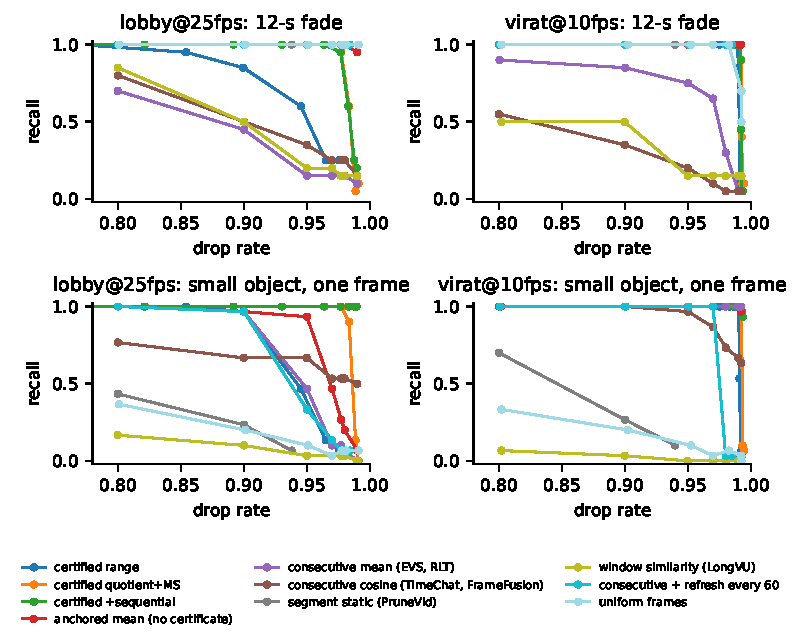
\includegraphics[width=\linewidth]{figures/audit_curves}
\caption{Recall of slow fades and of small objects against drop rate at the native frame rate, one panel per clip. Each curve is one rule swept over its threshold.}
\label{fig:auditcurves}
\end{figure}

\section{Computing the clairvoyant optimum}
\label{app:opt}

For one patch and a seminorm $\sigma$, $\OPT_\theta$ is the shortest sequence of keep times $0 = k_1 < k_2 < \dots$ such that every frame $t$ with anchor $k_j$ satisfies $\sigma(F_t - F_{k_j}) < \theta$. Let $\mathrm{reach}(k)$ be the last frame $t \ge k$ such that every frame in $[k, t]$ is within $\theta$ of $F_k$. A schedule is sound iff each keep's successor is at most $\mathrm{reach}(k) + 1$, so $\OPT_\theta$ is a shortest path on a DAG, computed by dynamic programming from the end of the sequence with $O(T^2)$ evaluations of $\sigma$ per patch. A brute-force search over all schedules confirms it on short random sequences. The anchored rule's keeps $m_\theta$ are counted on the same sequence, and Theorem~\ref{thm:opt}(i) and (ii) are checked on every patch (\texttt{scripts/competitive\_audit.py}).

\section{Reproducing the numbers}
\label{app:repro}

Every table and figure is generated from stored outputs by \texttt{scripts/make\_paper\_tables.py}. The outputs come from:

\begin{center}\scriptsize
\begin{tabular}{p{0.3\linewidth}p{0.62\linewidth}}
\toprule
result & command \\
\midrule
DAVIS (Table~\ref{tab:davis}) & \texttt{scripts/warp\_bench.py --davis all --frames 40} \\
film (Table~\ref{tab:film}) & \texttt{scripts/warp\_bench.py --film 120,360,540 --film-seconds 60} \\
synthetic audit (Table~\ref{tab:warpaudit}) & \texttt{scripts/warp\_audit.py} \\
competitive (Table~\ref{tab:competitive}) & \texttt{scripts/competitive\_audit.py --clips hall,lobby,virat --deltas 16,32,48} \\
shift cost (Table~\ref{tab:shift}) & \texttt{scripts/shift\_cost.py --clips hall,lobby,virat} \\
reducer audit (Tables~\ref{tab:audit}, \ref{tab:audit2fps}) & \texttt{scripts/audit\_reducers.py --clips lobby,virat --rates native,2} \\
\bottomrule
\end{tabular}
\end{center}

The theorems' finite claims are covered by \texttt{tests/test\_paper.py}: the fixed-camera parity of Appendix~\ref{app:parity}, registration of a synthetic pan, Theorem~\ref{thm:warp} against the constructed reference, the oscillation bound behind Proposition~\ref{prop:iota}, cut handling, Theorem~\ref{thm:opt}(i)--(ii) on random walks, optimality of the dynamic program by brute force, the adversary of Theorem~\ref{thm:opt}(iii), and Proposition~\ref{prop:consecutive} on a slow ramp for the re-implemented reducers. Footage is fetched by \texttt{scripts/fetch\_data.py}; DAVIS~2017 and Tears of Steel are under their own licences.
